\documentclass{standalone}
\usepackage{tikz}
\begin{document}
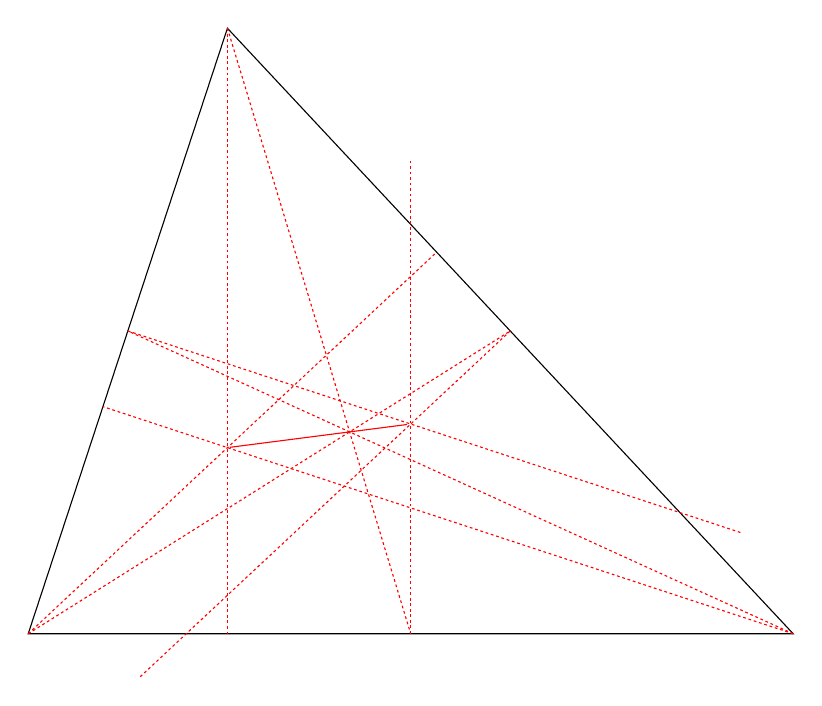
\begin{tikzpicture}[x=1pt,y=1pt]
\draw (14.18,-226.34) -- (290.58,-226.34) -- (86.16,-7.55) -- cycle;
\draw[red] (151.09,-150.74) -- (87.02,-158.99);
\draw[red, dash pattern=on 1pt] (86.16,-7.56) -- (152.38,-226.35);
\draw[red, dash pattern=on 1pt] (290.58,-226.35) -- (50.17,-116.94);
\draw[red, dash pattern=on 1pt] (14.18,-226.35) -- (188.38,-116.94);
\draw[red, dash pattern=on 1pt] (14.18,-226.35) -- (161.76,-88.47);
\draw[red, dash pattern=on 1pt] (290.58,-226.35) -- (41.17,-144.29);
\draw[red, dash pattern=on 1pt] (86.16,-7.56) -- (86.16,-226.35);
\draw[red, dash pattern=on 1pt] (188.38,-116.94) -- (54.45,-242.07);
\draw[red, dash pattern=on 1pt] (50.17,-116.94) -- (271.58,-189.78);
\draw[red, dash pattern=on 1pt] (152.38,-226.35) -- (152.38,-55.38);
\end{tikzpicture}
\end{document}
